\documentclass[tikz,border=6pt]{standalone}
\usepackage[T1]{fontenc}
\usepackage[utf8]{inputenc}
\usepackage{pgfplots}
\usepgfplotslibrary{groupplots}
\usetikzlibrary{calc}
\pgfplotsset{compat=1.18}
\begin{document}
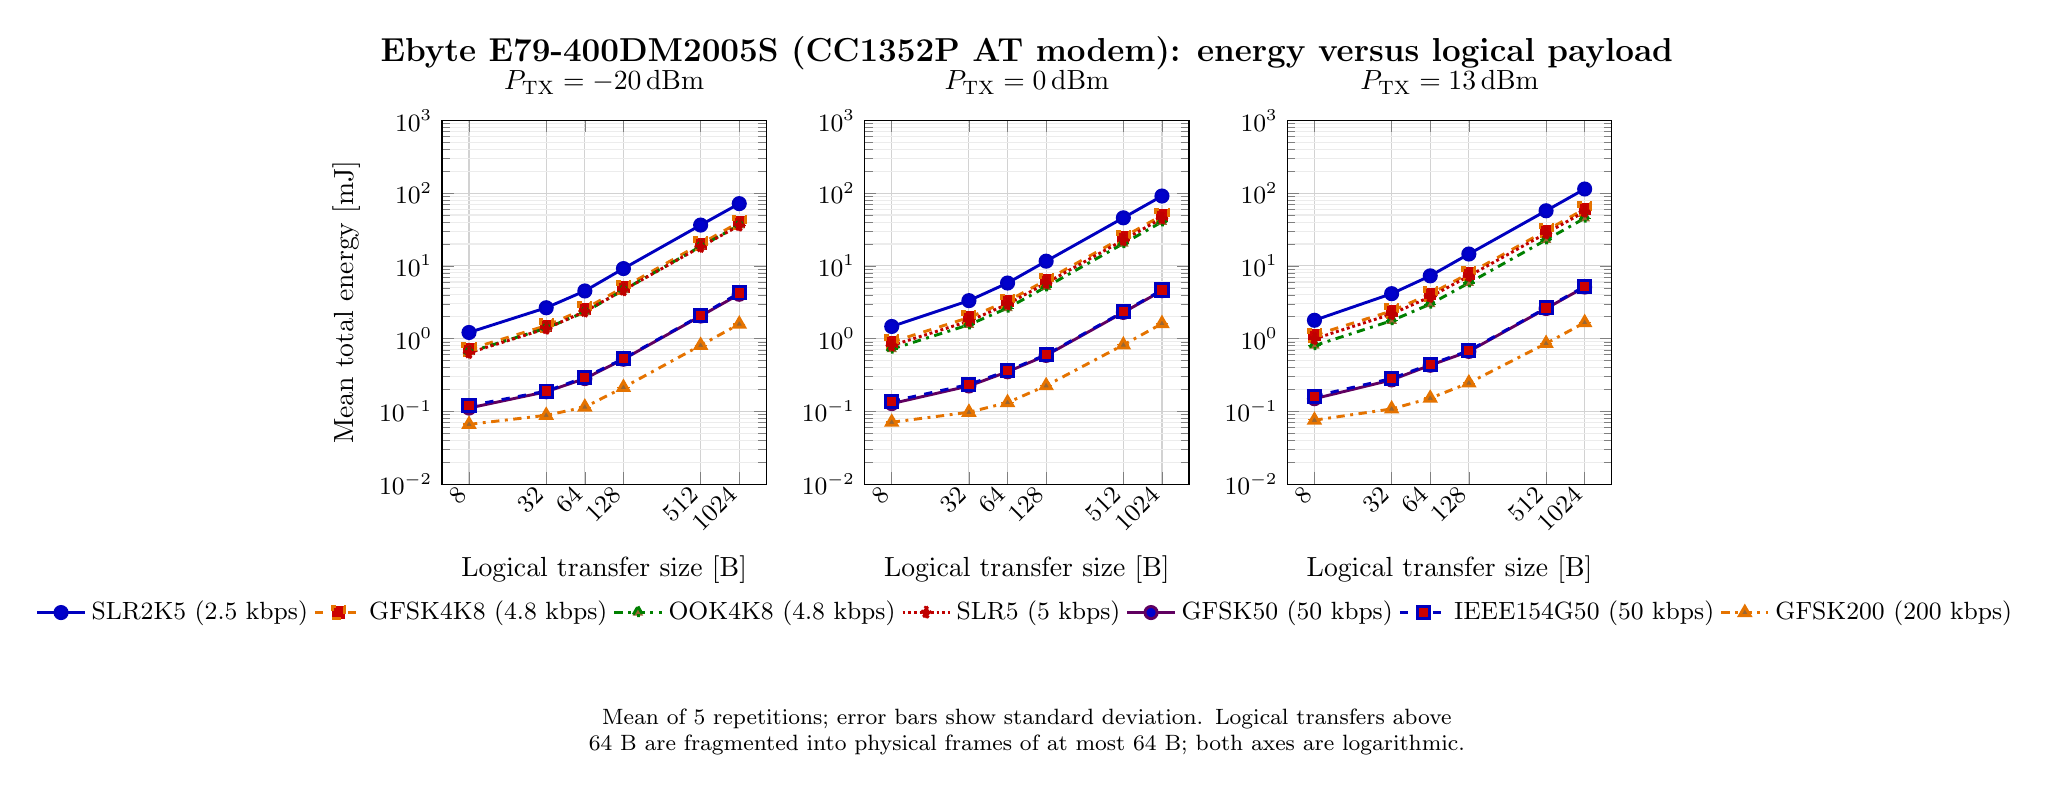
\begin{tikzpicture}
\begin{groupplot}[/pgf/number format/use comma,
  group style={group size=3 by 1, horizontal sep=1.25cm},
  width=5.7cm, height=6.2cm,
  xmode=log, log basis x={2}, ymode=log, log basis y={10},
  ymin=0.01, ymax=1000,
  xtick={8,32,64,128,512,1024}, xticklabels={8,32,64,128,512,1024},
  x tick label style={rotate=45, anchor=east, font=\small},
  y tick label style={font=\small},
  grid=both, minor grid style={gray!15}, major grid style={gray!35},
  xlabel={Logical transfer size [B]},
  every axis plot/.append style={line width=1.05pt},
  error bars/error bar style={line width=0.35pt},
  legend style={font=\small, draw=none, fill=none, at={(0.5,-0.29)},
    anchor=north, legend columns=-1},
]
\nextgroupplot[title={\(P_{\mathrm{TX}}=-20\,\mathrm{dBm}\)}, ylabel={Mean total energy [mJ]}]
\addplot+[
  color=blue!75!black, solid, mark=*, mark size=2.2pt,
  error bars/.cd, y dir=both, y explicit,
] coordinates {
  (8,1.21411135) +- (0,0.00327635652)
  (32,2.65612413) +- (0,0.00435279017)
  (64,4.51849776) +- (0,0.025823788)
  (128,9.18138285) +- (0,0.0149370122)
  (512,36.4216049) +- (0,0.035326064)
  (1024,71.7528464) +- (0,0.0962542646)
};
\addplot+[
  color=orange!90!black, dashed, mark=square*, mark size=2.2pt,
  error bars/.cd, y dir=both, y explicit,
] coordinates {
  (8,0.71458457) +- (0,0.00268867923)
  (32,1.50710529) +- (0,0.0032909662)
  (64,2.56373014) +- (0,0.00583314513)
  (128,5.06120534) +- (0,0.0140644025)
  (512,20.0462675) +- (0,0.0289057321)
  (1024,39.8990808) +- (0,0.071384026)
};
\addplot+[
  color=green!50!black, dashdotted, mark=triangle*, mark size=2.2pt,
  error bars/.cd, y dir=both, y explicit,
] coordinates {
  (8,0.653046649) +- (0,0.00273994109)
  (32,1.38933807) +- (0,0.0071703973)
  (64,2.31483831) +- (0,0.0100973238)
  (128,4.65838903) +- (0,0.0116259371)
  (512,18.5043522) +- (0,0.018318921)
  (1024,36.2287835) +- (0,0.0394886267)
};
\addplot+[
  color=red!75!black, densely dotted, mark=diamond*, mark size=2.2pt,
  error bars/.cd, y dir=both, y explicit,
] coordinates {
  (8,0.636832389) +- (0,0.0028430367)
  (32,1.37381263) +- (0,0.00722285221)
  (64,2.36218968) +- (0,0.0219889652)
  (128,4.63480298) +- (0,0.0140587866)
  (512,18.2747483) +- (0,0.0286156436)
  (1024,35.9133248) +- (0,0.0473813899)
};
\addplot+[
  color=violet!75!black, solid, mark=*, mark size=2.2pt,
  error bars/.cd, y dir=both, y explicit,
] coordinates {
  (8,0.11101693) +- (0,0.00131923625)
  (32,0.186003265) +- (0,0.00266160378)
  (64,0.281917829) +- (0,0.00164075496)
  (128,0.520538333) +- (0,0.00565738868)
  (512,2.04532992) +- (0,0.00431514131)
  (1024,4.07063123) +- (0,0.00836786337)
};
\addplot+[
  color=blue!75!black, dashed, mark=square*, mark size=2.2pt,
  error bars/.cd, y dir=both, y explicit,
] coordinates {
  (8,0.119271279) +- (0,0.00104723103)
  (32,0.189622481) +- (0,0.00125367288)
  (64,0.293280924) +- (0,0.00318672998)
  (128,0.529394826) +- (0,0.00443707034)
  (512,2.08592278) +- (0,0.00566566201)
  (1024,4.25375461) +- (0,0.00725394981)
};
\addplot+[
  color=orange!90!black, dashdotted, mark=triangle*, mark size=2.2pt,
  error bars/.cd, y dir=both, y explicit,
] coordinates {
  (8,0.0661925189) +- (0,0.000764915303)
  (32,0.0881610944) +- (0,0.00135404779)
  (64,0.114374429) +- (0,0.000496302015)
  (128,0.212973801) +- (0,0.00121852336)
  (512,0.807841227) +- (0,0.00164090333)
  (1024,1.58757286) +- (0,0.003065327)
};
\nextgroupplot[title={\(P_{\mathrm{TX}}=0\,\mathrm{dBm}\)}]
\addplot+[
  color=blue!75!black, solid, mark=*, mark size=2.2pt,
  error bars/.cd, y dir=both, y explicit,
] coordinates {
  (8,1.46884739) +- (0,0.00420132974)
  (32,3.32803035) +- (0,0.00477648587)
  (64,5.80976781) +- (0,0.00824971836)
  (128,11.60445) +- (0,0.0293493548)
  (512,45.8096739) +- (0,0.0682636088)
  (1024,91.3126604) +- (0,0.064720616)
};
\addlegendentry{SLR2K5 (2.5 kbps)}
\addplot+[
  color=orange!90!black, dashed, mark=square*, mark size=2.2pt,
  error bars/.cd, y dir=both, y explicit,
] coordinates {
  (8,0.897786779) +- (0,0.0033538482)
  (32,1.94921188) +- (0,0.00463335513)
  (64,3.27710745) +- (0,0.00880519488)
  (128,6.35767081) +- (0,0.00951563768)
  (512,24.8208221) +- (0,0.0576793571)
  (1024,49.4618915) +- (0,0.0374113041)
};
\addlegendentry{GFSK4K8 (4.8 kbps)}
\addplot+[
  color=green!50!black, dashdotted, mark=triangle*, mark size=2.2pt,
  error bars/.cd, y dir=both, y explicit,
] coordinates {
  (8,0.716277476) +- (0,0.00185039751)
  (32,1.55042146) +- (0,0.0034599729)
  (64,2.62891584) +- (0,0.00850120846)
  (128,5.14134751) +- (0,0.00956474329)
  (512,20.2812527) +- (0,0.0318528951)
  (1024,40.2660583) +- (0,0.03949167)
};
\addlegendentry{OOK4K8 (4.8 kbps)}
\addplot+[
  color=red!75!black, densely dotted, mark=diamond*, mark size=2.2pt,
  error bars/.cd, y dir=both, y explicit,
] coordinates {
  (8,0.803577765) +- (0,0.00327985484)
  (32,1.73836115) +- (0,0.00350245529)
  (64,2.98074016) +- (0,0.00669592039)
  (128,5.80045754) +- (0,0.0269934985)
  (512,22.6370252) +- (0,0.0621319626)
  (1024,45.1107835) +- (0,0.0451794307)
};
\addlegendentry{SLR5 (5 kbps)}
\addplot+[
  color=violet!75!black, solid, mark=*, mark size=2.2pt,
  error bars/.cd, y dir=both, y explicit,
] coordinates {
  (8,0.127808566) +- (0,0.000877761957)
  (32,0.223285523) +- (0,0.000836756555)
  (64,0.349895741) +- (0,0.000932275)
  (128,0.587085289) +- (0,0.00174447637)
  (512,2.29230497) +- (0,0.00709364098)
  (1024,4.55753175) +- (0,0.0090038604)
};
\addlegendentry{GFSK50 (50 kbps)}
\addplot+[
  color=blue!75!black, dashed, mark=square*, mark size=2.2pt,
  error bars/.cd, y dir=both, y explicit,
] coordinates {
  (8,0.137431071) +- (0,0.000947579065)
  (32,0.234149859) +- (0,0.00153989844)
  (64,0.360938718) +- (0,0.00211486696)
  (128,0.601354208) +- (0,0.000711682913)
  (512,2.33923961) +- (0,0.0376790593)
  (1024,4.65667417) +- (0,0.0109417497)
};
\addlegendentry{IEEE154G50 (50 kbps)}
\addplot+[
  color=orange!90!black, dashdotted, mark=triangle*, mark size=2.2pt,
  error bars/.cd, y dir=both, y explicit,
] coordinates {
  (8,0.0707942785) +- (0,0.000546131213)
  (32,0.0971460833) +- (0,0.000585329404)
  (64,0.131926193) +- (0,0.00135639949)
  (128,0.225248822) +- (0,0.000609839933)
  (512,0.818798099) +- (0,0.00108609021)
  (1024,1.60794684) +- (0,0.0150222952)
};
\addlegendentry{GFSK200 (200 kbps)}
\nextgroupplot[title={\(P_{\mathrm{TX}}=13\,\mathrm{dBm}\)}]
\addplot+[
  color=blue!75!black, solid, mark=*, mark size=2.2pt,
  error bars/.cd, y dir=both, y explicit,
] coordinates {
  (8,1.78682554) +- (0,0.00193720275)
  (32,4.14961761) +- (0,0.00643593785)
  (64,7.29493148) +- (0,0.0126967254)
  (128,14.5605686) +- (0,0.0379098161)
  (512,57.2527543) +- (0,0.0602916345)
  (1024,114.028554) +- (0,0.117074788)
};
\addplot+[
  color=orange!90!black, dashed, mark=square*, mark size=2.2pt,
  error bars/.cd, y dir=both, y explicit,
] coordinates {
  (8,1.11575312) +- (0,0.00299768886)
  (32,2.39937627) +- (0,0.00648337206)
  (64,4.10935177) +- (0,0.00687165253)
  (128,7.85627879) +- (0,0.024885918)
  (512,30.5631105) +- (0,0.0526300401)
  (1024,60.6147494) +- (0,0.113818251)
};
\addplot+[
  color=green!50!black, dashdotted, mark=triangle*, mark size=2.2pt,
  error bars/.cd, y dir=both, y explicit,
] coordinates {
  (8,0.801347946) +- (0,0.00269755522)
  (32,1.76326219) +- (0,0.00670972562)
  (64,2.98277785) +- (0,0.00281687772)
  (128,5.83050029) +- (0,0.0116424233)
  (512,22.762573) +- (0,0.0211711607)
  (1024,45.2156346) +- (0,0.0618876963)
};
\addplot+[
  color=red!75!black, densely dotted, mark=diamond*, mark size=2.2pt,
  error bars/.cd, y dir=both, y explicit,
] coordinates {
  (8,0.992945309) +- (0,0.0015784517)
  (32,2.17604681) +- (0,0.00314660668)
  (64,3.7570602) +- (0,0.00369477244)
  (128,7.25109863) +- (0,0.027072279)
  (512,28.0706404) +- (0,0.060897947)
  (1024,55.6383125) +- (0,0.119776105)
};
\addplot+[
  color=violet!75!black, solid, mark=*, mark size=2.2pt,
  error bars/.cd, y dir=both, y explicit,
] coordinates {
  (8,0.149257074) +- (0,0.000998008295)
  (32,0.270372655) +- (0,0.00110112891)
  (64,0.430289998) +- (0,0.00221702985)
  (128,0.666311061) +- (0,0.000866845194)
  (512,2.59209225) +- (0,0.0115005492)
  (1024,5.11540087) +- (0,0.00783537147)
};
\addplot+[
  color=blue!75!black, dashed, mark=square*, mark size=2.2pt,
  error bars/.cd, y dir=both, y explicit,
] coordinates {
  (8,0.161736921) +- (0,0.000876658039)
  (32,0.282554274) +- (0,0.00196616361)
  (64,0.443979802) +- (0,0.00131216071)
  (128,0.682422789) +- (0,0.00221809947)
  (512,2.63993299) +- (0,0.0357372308)
  (1024,5.22479192) +- (0,0.010542337)
};
\addplot+[
  color=orange!90!black, dashdotted, mark=triangle*, mark size=2.2pt,
  error bars/.cd, y dir=both, y explicit,
] coordinates {
  (8,0.0756527262) +- (0,0.000878431519)
  (32,0.10788161) +- (0,0.00118107306)
  (64,0.151540968) +- (0,0.00101543015)
  (128,0.245744313) +- (0,0.00107293936)
  (512,0.85730023) +- (0,0.0013454389)
  (1024,1.66032186) +- (0,0.0082014162)
};
\end{groupplot}
\node[font=\bfseries\large] at ($(group c2r1.north)+(0,0.85cm)$)
  {Ebyte E79-400DM2005S (CC1352P AT modem): energy versus logical payload};
\node[font=\footnotesize, align=center, text width=18.5cm]
  at ($(group c2r1.south)+(0,-3.15cm)$)
  {Mean of 5 repetitions; error bars show standard deviation. Logical transfers above 64 B are fragmented into physical frames of at most 64 B; both axes are logarithmic.};
\end{tikzpicture}
\end{document}
